\chapter{Antecedentes}
\label{chap:antecedentes}

%Este capítulo incluye unas nociones básicas de \LaTeX{} y algunos consejos
%sencillos de composición para sacar todo el jugo a la clase \esitfg. Ten
%presente que este capítulo está pensado para que leas el código fuente y lo
%compares con el resultado en PDF.

\drop{E}{n} este capítulo se muestra el trabajo de documentación e investigación previa a la realización del presente \ac{TFG}. En primer lugar se abordarán los sistemas de posicionamiento, su historia y el desarrollo del 

gps\footnote{Debido al extendido uso de la denominación \textit{GPS} como sinónimo de los \ac{GNSS}, se usará de este modo. Para referirse al sistema de posicionamiento propiedad del gobierno de los Estados Unidos \acf{GPS} se utilizará el acrónimo en mayúsculas} 

y los antecedentes de los \ac{SIG}, más tarde se comentarán algunos aspectos relevantes de las tecnologías web y móviles. Para terminar, se enumerarán algunas aplicaciones similares que podemos encontrar actualmente en el mercado.

\section{Localización geográfica y \acf{SIG}}

%HISTORIA DEL GPS
Los \ac{GNSS} permiten conocer en tiempo real la posición de un objeto cualquiera en la superficie terrestre.

Según Scott Gleason y Demoz Gebre-Egziabher \cite{Glea09} podríamos definir la navegación como:

\begin{tikzpicture}
	\node[shadowBox] {El proceso de determinación de la posición, la velocidad y, en algunos casos, la orientación de un objeto.};
\end{tikzpicture}

Por tanto, un \ac{GNSS} consiste en una constelación de satélites que permiten determinar con precisión las coordenadas geográficas y la altitud de un punto dado en cualquier punto de la superficie terrestre.

El inicio de este tipo de sistemas podríamos encontrarlo en los primeros marinos. La decisión de alejarse de las rutas que transcurrían a lo largo de la línea de visión de la costa, con la intención de reducir el tiempo, los costes derivados de los viajes y la posibilidad de encontrar nuevos mercados, planteó un nuevo reto tecnológico consistente en conocer con exactitud la localización en la que se encontraban.
La primera solución vino de la mano de un gran conocimiento de la bóveda celeste y la posición de las estrellas. Usando instrumentos como el astrolabio y el sextante (ver figura \ref{fig:sextante_astrolabio}), se podía calcular con asombrosa exactitud la posición.

\begin{figure}[hbtp]
	\begin{adjustbox}{minipage=\linewidth, fbox}
		\centering
		\subfigure[Sextante]{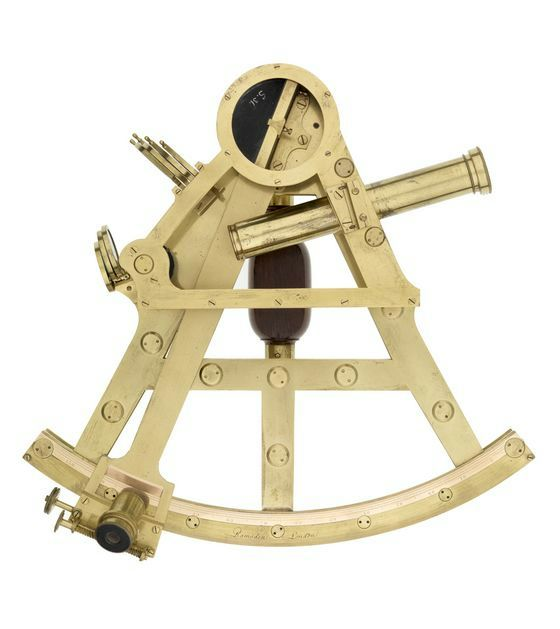
\includegraphics[width=60mm, height=80mm]{./images/03-antecedentes/04-sextante.png}}
		\hspace{10mm}
		\subfigure[Astrolabio]{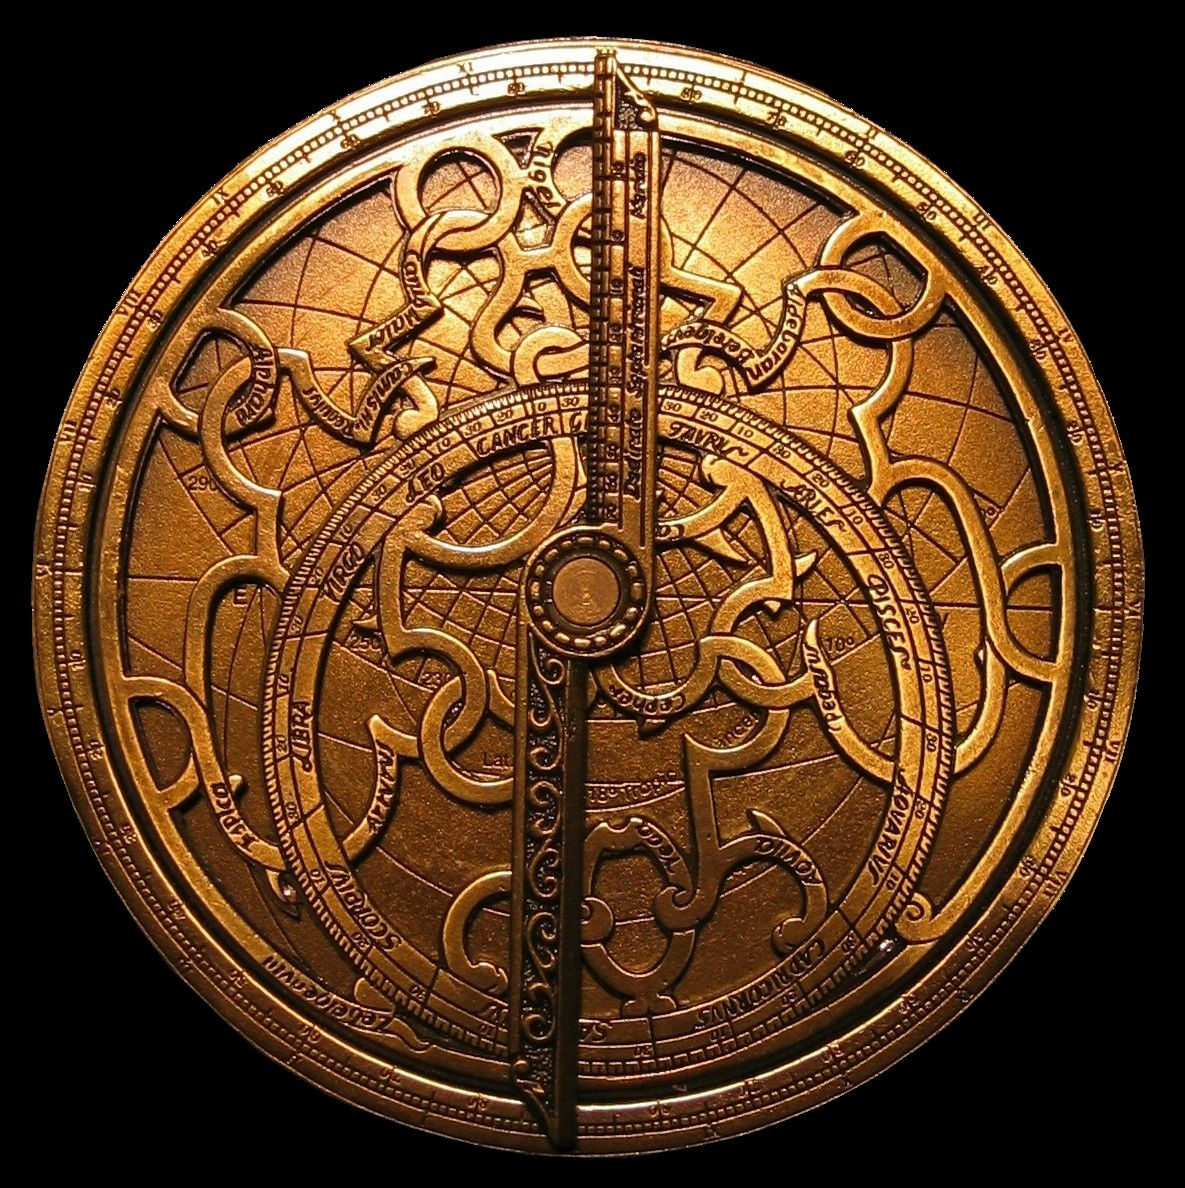
\includegraphics[height=80mm]{./images/03-antecedentes/05-astrolabio.png}}
	\end{adjustbox}
	\caption{Primeros instrumentos de navegación}
	\label{fig:sextante_astrolabio}
\end{figure}

Hasta tiempos recientes (segunda mitad del S. XX), con la irrupción del geoposicionamiento satelital, este era el método usado para conocer la ubicación en la que se encontraban.
Los primeros prototipos del gps se desarrollan a principios del S. XX, coincidiendo con los comienzos de la automoción, aspecto este último que ha dado la gran fama a esta tecnología.
El primer gps data de 1909, que consistía en un odómetro que giraba un mapa indicando los hitos más importantes que se podían encontrar en el punto kilométrico en el que estabas.
Este primer prototipo se llamaba \textit{Jones Live Map} (ver figura \ref{fig:jones_live_map}), cada mapa era válido para unos 160 km y después había que cambiarlo por el siguiente mapa. Este primer intento dejó de fabricarse en los años 20, cuando las carreteras estaban correctamente señalizadas\cite{jones_live_map}.

\begin{figure}[hbtp]
\centering
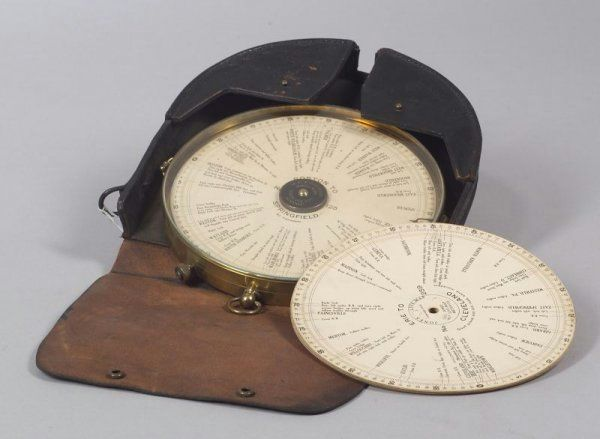
\includegraphics[scale=0.5, fbox={\fboxrule} 4mm]{images/03-antecedentes/06-jones_live_map.png}
\caption{Jones Live Map}
\label{fig:jones_live_map}
\end{figure}

También en la década de los veinte, hizo su aparición el \textit{Plus Fours Routefinder} (ver figura \ref{fig:plus_fours_routefinder}), consistente en un pequeño reloj de muñeca con una serie de papiros con la información de la ruta que debían ir desenrollándose de forma manual para ir viendo las indicaciones\cite{plus_fours_routefinders}.

\begin{figure}[hbtp]
\centering
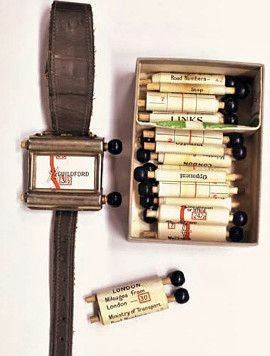
\includegraphics[scale=0.5, fbox={\fboxrule} 4mm]{images/03-antecedentes/07-plus_fours_routefinder.png}
\caption{Plus Fours Routefinder}
\label{fig:plus_fours_routefinder}
\end{figure}

Otro de los padres del gps moderno es el llamado \textit{Iter Avto} (ver figura \ref{fig:iter_avto}), consistente en un mapa enrollado conectado al velocímetro del coche para sincronizarlo. La dos grandes ventajas con respecto al \textit{Plus Fours Routefinder}, consistía en que se instalaba sobre el salpicadero del coche y mostraba de forma gráfica la posición. Su inconveniente, cualquier desviación de la ruta era completamente indetectable\cite{iter_avto}.

\begin{figure}[hbtp]
\centering
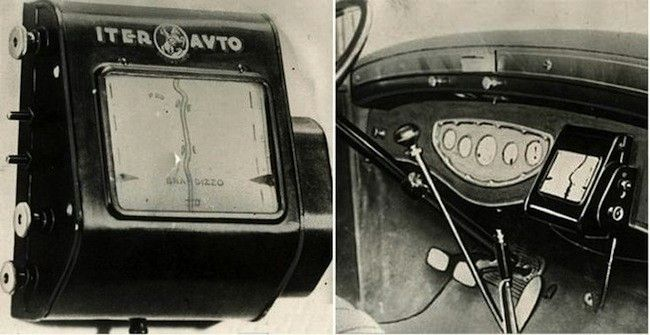
\includegraphics[scale=0.5, fbox={\fboxrule} 4mm]{images/03-antecedentes/08-iter_avto.png}
\caption{Iter Avto}
\label{fig:iter_avto}
\end{figure}

Durante la segunda guerra mundial, la \ac{RAF} desarrolló un sistema de
posicionamiento para sus bombarderos consistente en tres estaciones de radar que localizaban
con precisión al avión\cite{raf}.
Los verdaderos orígenes de los gps como sistema de navegación satelital se remontan a 1957 con
el programa \textit{TRANSIT}. Por un lado la marina de los estados unidos inicia el programa \textit{Polaris},
que consiste en el despliegue de misiles intercontinentales suboceánicos. Alcanzar los objetivos
con los misiles dependía de la capacidad de determinar con precisión la posición de los
submarinos en cualquier punto de la superficie terrestre. Por otro lado, la universidad Johns
Hopking de Maryland, consigue determinar con precisión la órbita del \textit{Sputnik 1} a partir del
desplazamiento Doppler sufrido por la señal que emitía y el conocimiento preciso de la posición
del receptor. Con estos elementos, invertir los términos del problema resultó relativamente
sencillo, esto es, conociendo la posición de un satélite de forma precisa, es posible determinar
la de un receptor situado en el submarino de posición desconocida midiendo el desplazamiento
Doppler sufrido por la señal emitida del satélite.

El sistema \textit{TRANSIT} entró en funcionamiento en 1964 con el lanzamiento de 10 satélites y se mantuvo en servicio
hasta 1996. En 1967 se permitió su uso civil. El error típico de este sistema era de unos 250
metros, por lo que resultaba muy útil para la navegación de aviones, barcos y submarinos, pero
por razones obvias (precisión y tamaño de los receptores) aún estaban lejos de los sistemas de
navegación personal actuales.

La Unión Soviética había desarrollado casi al mismo tiempo, un sistema muy parecido con
idénticas prestaciones, el \textit{TSICADA}, lo que resultaba inadmisible para los norteaméricanos en el
contexto de la guerra fría, por lo que comenzó a desarrollarse lo que posteriormente sería el
\ac{GPS}\cite{tsicada}.
El \textit{NAVSTAR-GPS} nació en 1973 para uso exclusivamente militar, con una constelación de 24
satélites en órbitas inclinadas de 12 horas, lo que se traducía en que cualquier receptor en el
mundo tendría en su horizonte visible al menos 5 satélites disponibles en todo momento. El
TRANSIT, no sólo no podía garantizar esto, debido a que sus satélites eran de órbita baja, si no
que con sus 6 satélites, algunos receptores podían estar varias horas esperando señal. El primer
satélite se puso en órbita en 1978. La precisión de este nuevo sistema era de 1 metro y podía
ser incorporado en misiles, bombas inteligentes, vehículos, etc. Debido a su consideración de
recurso de gran valor estratégico, su uso estaba limitado al ámbito estrictamente militar.
El 31 de agosto de 1983 tuvo lugar uno de los incidentes internacionales más graves de la
guerra fría, que a la postre resultaría decisivo para el uso actual del \ac{GPS}, el derribo del vuelo de
\textit{Korean Airlines KAL007} por parte de la \ac{URSS}\cite{007_korean}.

El citado vuelo, usando los sistemas de navegación tradicionales disponibles en aquella época, y
usando el piloto automático, invadió en dos ocasiones el espacio aéreo de la Unión Soviética,
que acabó interceptándolo mediante dos cazas militares y derribándolo con un ataque con
misiles, matando al pasaje y la tripulación completa, con un resultado de 269 fallecidos.
La respuesta internacional no se hizo esperar, y el entonces presidente de \ac{USA}, Ronald Reagan,
anunció que el sistema \ac{GPS} estaría disponible para propósitos civiles una vez finalizase el
proyecto, con la intención de que no se volvieran a repetir incidentes similares.
Para evitar que sus enemigos pudieran hacer uso de esta nueva tecnología para construir
misiles de precisión con los que atacarlos, el Departamento de Defensa de \ac{EE.UU.} impuso una
serie de restricciones en la precisión de los receptores, de manera que el error en el
posicionamiento fuera mayor que el de los disponibles para uso militar. Por ello los receptores de gps de uso
civil eran incapaces de mostrar una resolución menor de 20 metros.
Durante la primera guerra del golfo, en 1991, se desarrolló una mejora en la precisión del \ac{GPS}
llamada, \ac{GPS} Diferencial, que conseguía precisiones de entre 1 y 3 metros de exactitud.



%HISTORIA DEL SIG
Debido a que el término \ac{SIG} engloba la integración de muy diversas áreas,no existe una única definición totalmente consensuada\cite{Chr97}. La definición aportada por el \ac{NCGIA} resulta ampliamente aceptada:
\begin{tikzpicture}
	\node[shadowBox] {
	Un SIG es un sistema de hardware, software y procedimientos elaborados para facilitar la obtención, gestión, manipulación, análisis, modelado, representación y salida de datos espacialmente referenciados, para resolver problemas complejos de planificación y gestión.};
\end{tikzpicture}

Uno de los elementos relevantes de los \ac{SIG} son la asociación de información a una imagen concreta y una de las primeras muestras de esto lo podemos encontrar en el Londres victoriano de mediados del siglo XIX. En el año 1854, el doctor John Snow (ver figura \ref{fig:john_snow}) utilizó un mapa del Soho londinense para ubicar los casos de un brote de cólera (ver figura \ref{fig:cholera_map}). Con la ayuda de los registros del hospital de Middlesex y de Henry Whitehead, párroco local, recogió las defunciones producidas mediante una fina línea de color negro que se apilaban unas sobre otras a medida que se producían las muertes, consiguiendo el efecto de asociación de información a imagen comentado en el párrafo anterior \cite{Cai11}.

Este ejemplo temprano, combinado con la geolocalización nos permite identificar las líneas base de representación de lo que será el presente \ac{TFG}.

\begin{figure}[hbtp]
\centering
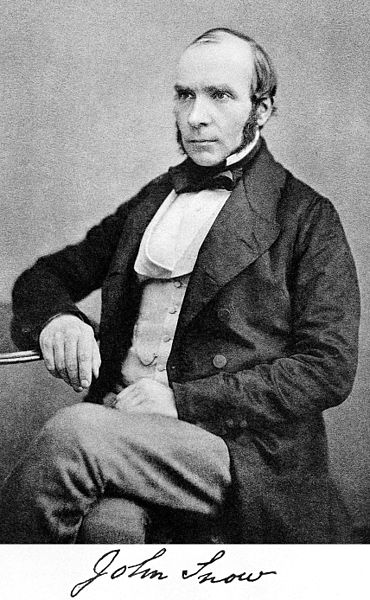
\includegraphics[scale=1, fbox={\fboxrule} 0mm]{images/03-antecedentes/02-john_snow.jpg}
\caption{Doctor Sir John Snow}
\label{fig:john_snow}
\end{figure}

\begin{figure}[hbtp]
\centering
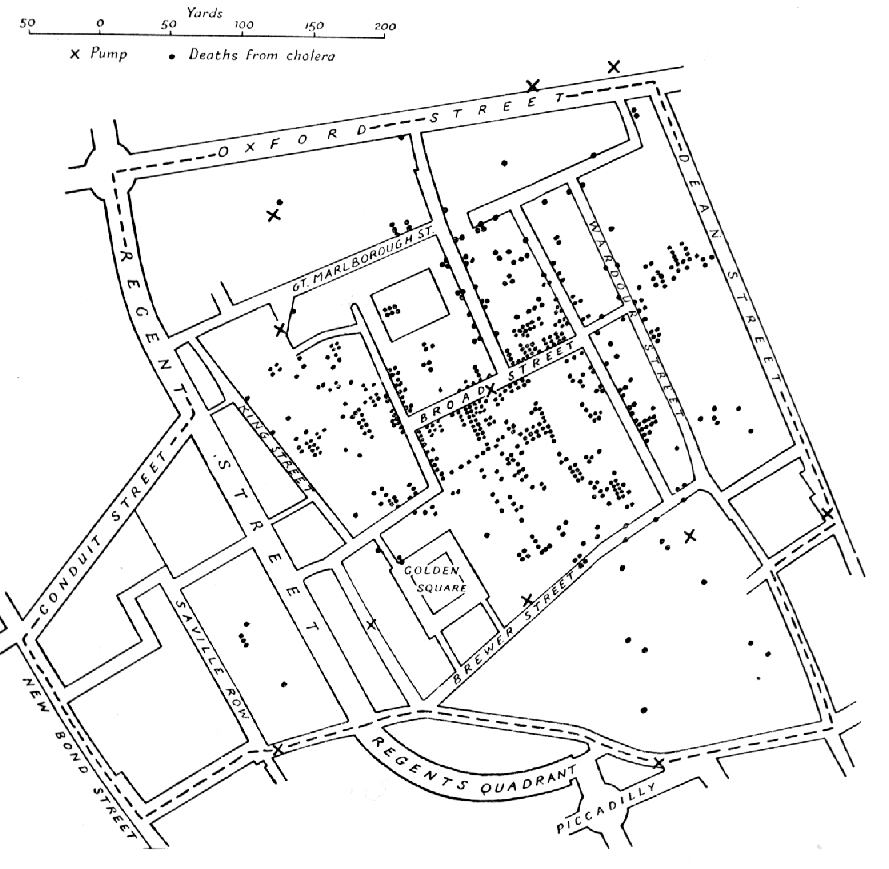
\includegraphics[scale=0.5, fbox={\fboxrule} 4mm]{images/03-antecedentes/01-cholera_map.jpg}
\caption{Mapa del Soho con los casos de fallecimiento por cólera}
\label{fig:cholera_map}
\end{figure}

Gracias a ello y referenciando en el mapa la posición de los pozos de agua, pudo comprobar como una gran cantidad de víctimas se encontraban dentro de la zona de influencia de una bomba de agua en Broad Street (ver figura \ref{fig:cholera_map_detail}), que a la postre resultó estar contaminada con heces. Recomendando la clausura de la misma consiguió acabar con la epidemia \cite{Gunn07}. Debido a estos logros se le considera el padre de la epidemiología moderna y podemos ilustrar uno de los primeros ejemplos del uso de los \ac{SIG}.

\begin{figure}[hbtp]
\centering
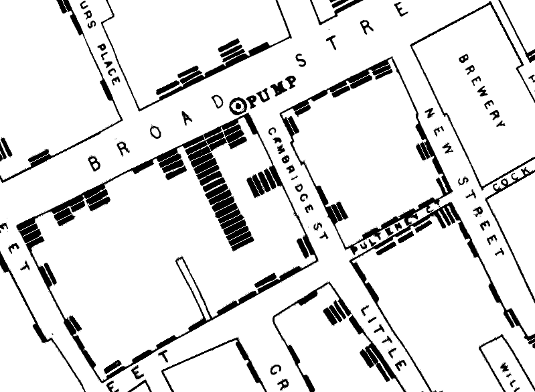
\includegraphics[scale=0.5, fbox={\fboxrule} 4mm]{images/03-antecedentes/03-cholera_map_detail.png}
\caption{Detalle del mapa del Doctor Snow}
\label{fig:cholera_map_detail}
\end{figure}

\section{Tecnologías web}

\section{Dispositivos móviles}

\section{Aplicaciones similares}



% Local Variables:
%  coding: utf-8
%  mode: latex
%  mode: flyspell
%  ispell-local-dictionary: "castellano8"
% End:
